\section{Results}
\label{sec:results}
Simulations are first run on a simpler map to test the system's navigation features, being the assignment of the exploration goal and the generation of a feasible path. Following, a more complex environment is selected to visualize the correctness of the reconstructed point cloud.
We initially deploy two robots in the \textit{Turtlebot3 stage 4} world \cite{turtlebot3-simulation}. The agents are capable of autonomously navigate through the environment, continuously exploring the detected frontiers and updating the global map. In Figure \ref{fig:path}, it can be observed how smooth paths are generated, connecting the robot with the frontier with most reward.

\begin{figure}[h]
  \begin{center}
    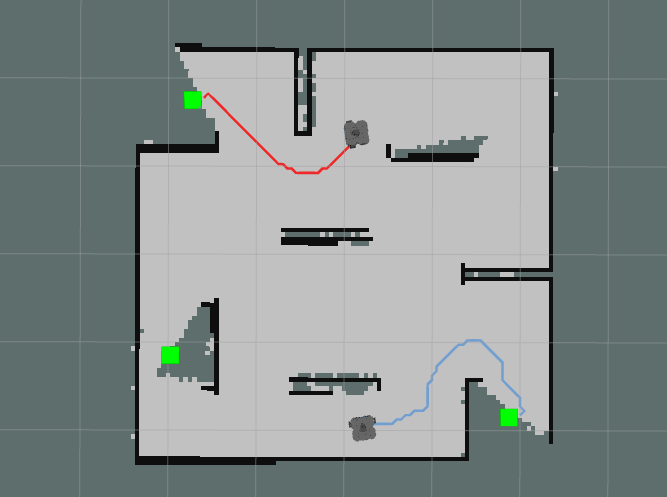
\includegraphics[width=0.4\textwidth]{img/path.png}
  \end{center}
  \caption[]{
    \textbf{Paths generated combining A* with FMM.} 
    Green squares represent the detected frontiers.
  }
  \label{fig:path}
\end{figure}

We now move to analyzing the efficiency of the exploration strategy. We will compare a strategy which uses reward function only based on the distance robot-frontier, and one where the information gain is added.
10 simulations are run with each strategy, and the mean and standard deviation of the explored area overtime are reported. Initial 2D poses for the robots, in terms of (x, y, yaw), are set to $[-0.3, -0.5, \pi/2]$ and $[-1, -0.5, \pi/2]$. The vehicle control policy, in terms of linear and angular acceleration, is kept the same for both strategies.
In Figure \ref{fig:results}, the explored area (in $m^2$) is compared with respect to the time required to map it.
\begin{figure}[b]
  \begin{center}
    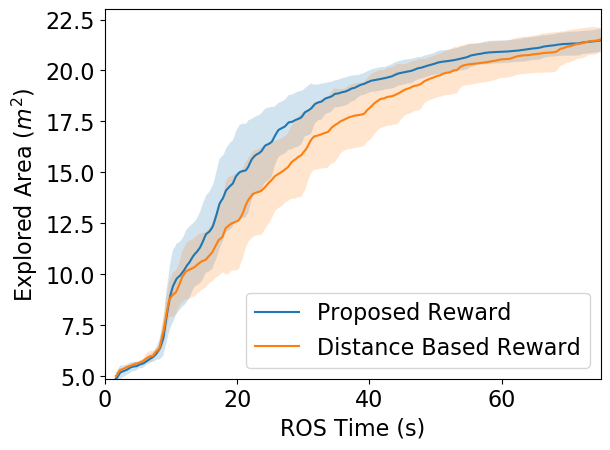
\includegraphics[width=0.49\textwidth]{img/mapping_speed.png}
  \end{center}
  \caption[]{
    \textbf{Exploration Strategy Results.} 
  }
  \label{fig:results}
\end{figure}
As it can be observed, both reward functions typically result in comprehensive map exploration within a similar timeframe. However, the introduction of information gain significantly expedites the initial phases of exploration. Initially, the robot will prioritize large frontiers, leaving smaller areas as unexplored. In this way, it is possible to rapidly obtain a rough version of the map, where most of the macro-regions have been explored. While this behavior proves effective in simpler maps, it may lead to reduced efficiency in more complex environments. For larger spaces, complete exploration may take longer, as nearby frontiers are deprioritized and revisited only much later. Consequently, this approach necessitates fine-tuning of the exploration gain based on the specific map.

Moving forward, we analyze the quality of the point cloud depending on the approaches proposed in the Section \ref{sec:point_cl}.
Regarding the merged point clouds, there is minimal or no difference between the results obtained with the online and offline solutions. This is due to the fact that the initial guess for the initial pose of the robots was accurate, therefore in the end there is minimal or no roto-translation between the two results. The final merged point cloud can be seen in Figure \ref{fig:merged}, where the standard \textit{Home} world from the Turtlebot3 project was used for the simulation \cite{turtlebot3-simulation}. 

\begin{figure}[H]
  \begin{center}
    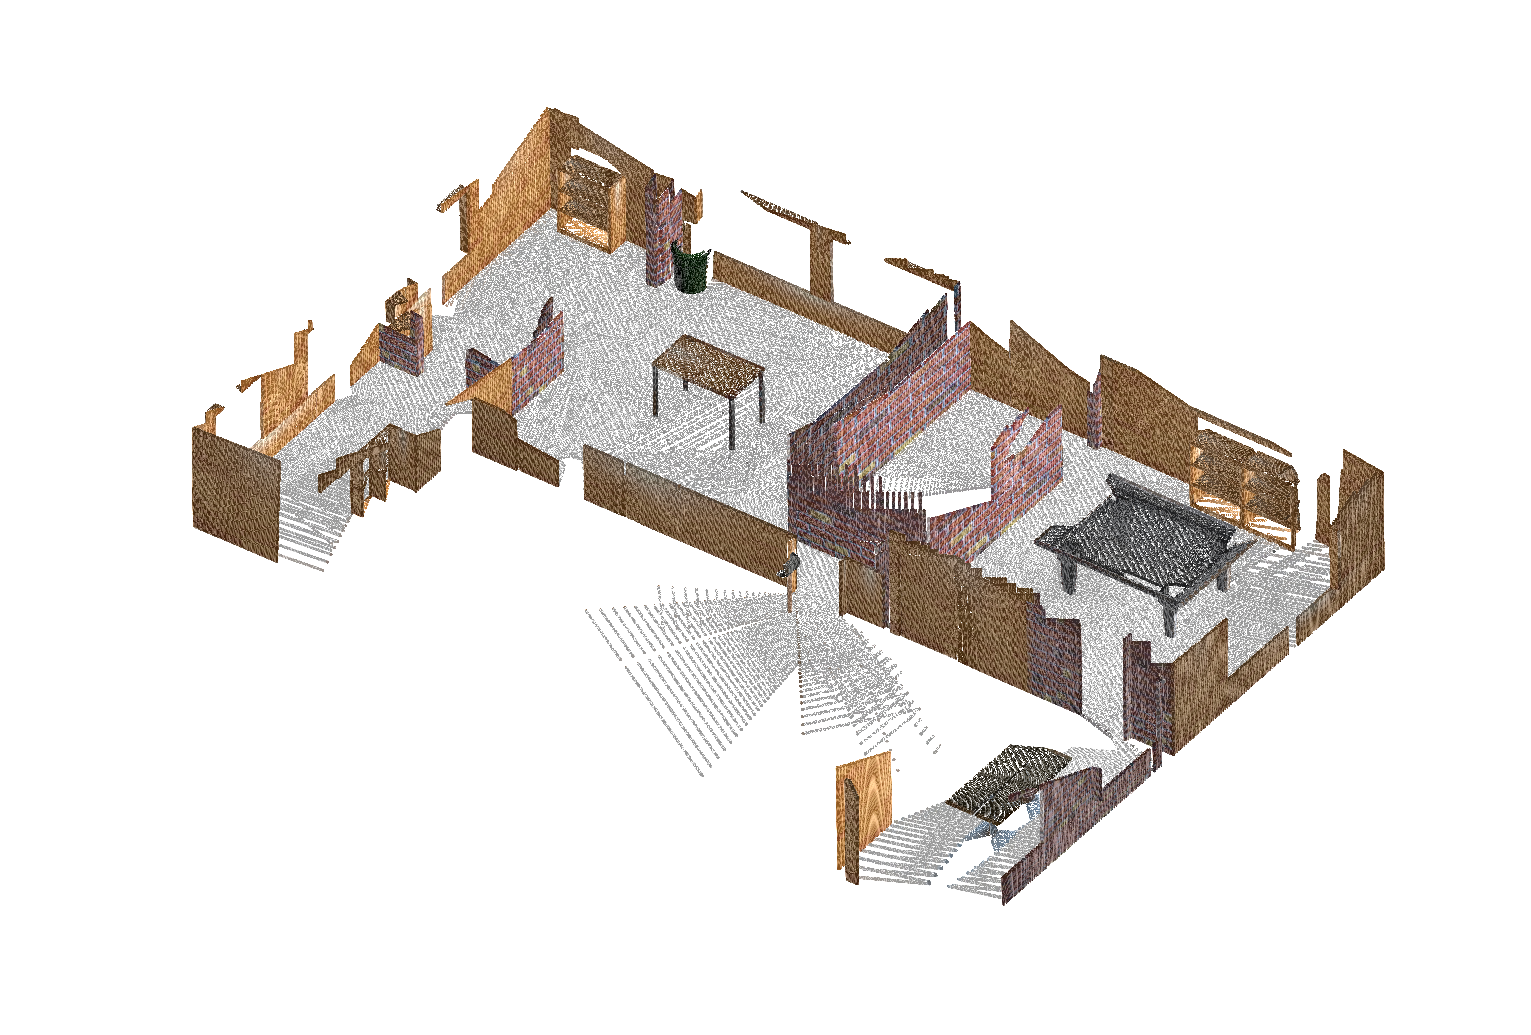
\includegraphics[width=0.49\textwidth]{img/merged.png}
  \end{center}
  \caption[]{
    \textbf{Final merged map} 
  }
  \label{fig:merged}
\end{figure}

Focusing more on the result obtained with the offline algorithm, in Figure \ref{fig:split} it is possible to see the two halves of the merged point cloud, that come from the two instances of RTAB-Map used during the simulation. 

\begin{figure}[H]
  \begin{center}
    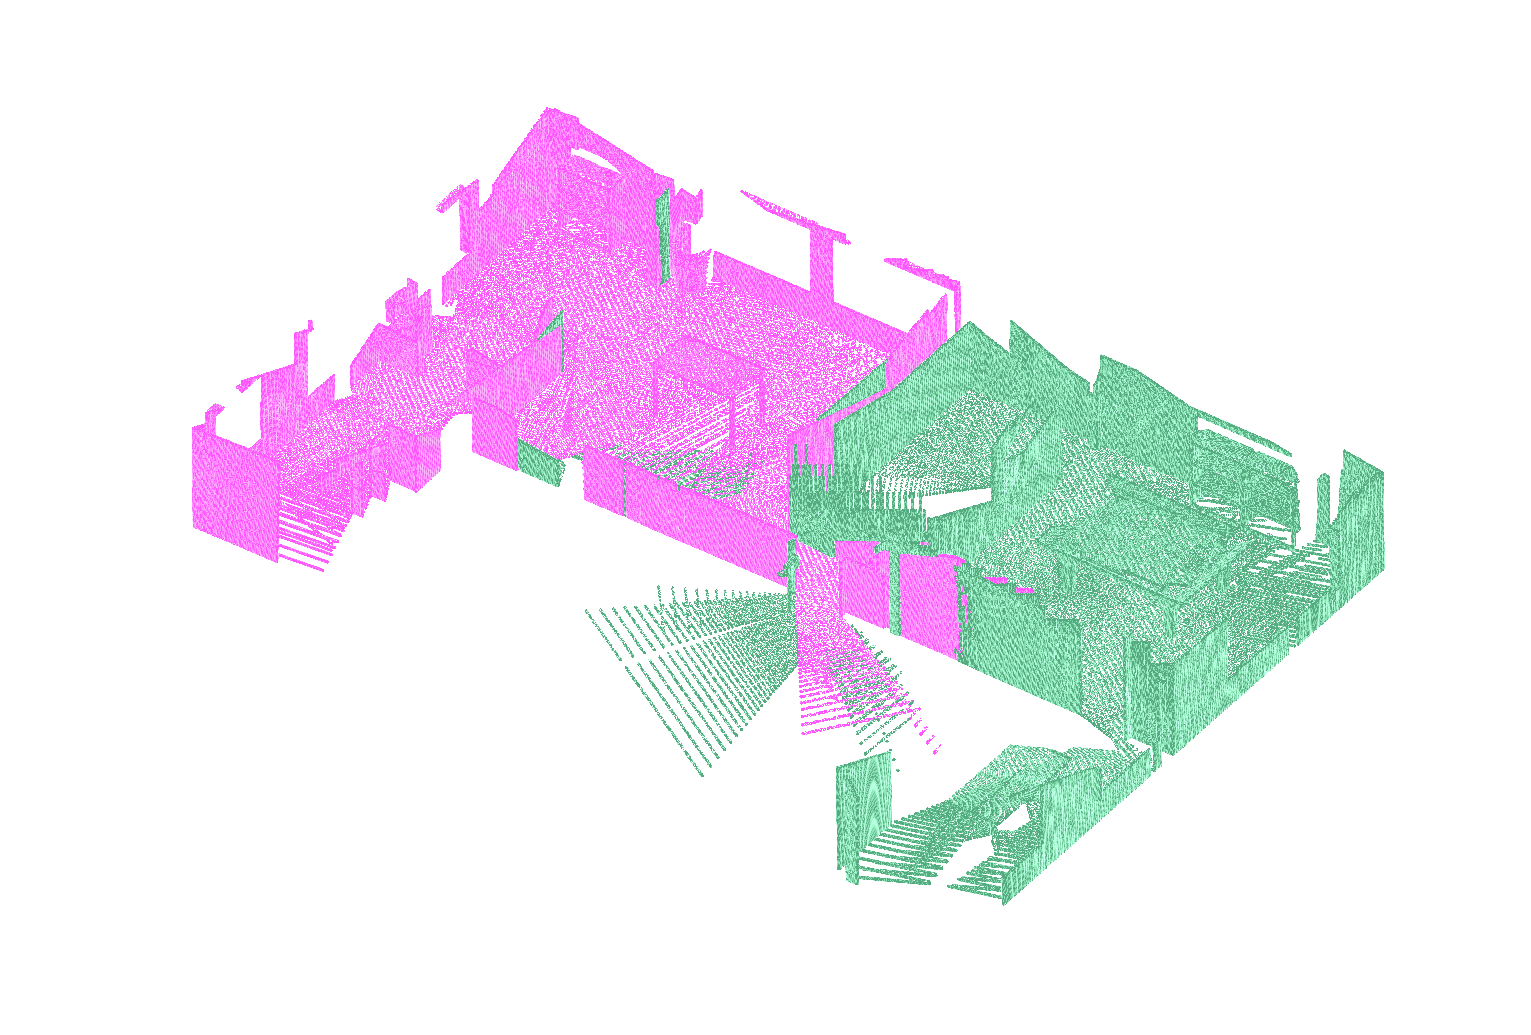
\includegraphics[width=0.49\textwidth]{img/split.png}
  \end{center}
  \caption[]{
    \textbf{Maps merged to form the final map} 
  }
  \label{fig:split}
\end{figure}

Finally, in Figure \ref{fig:example}, it is possible to see how the points shared between the two point clouds are handled by the algorithm. It can be observed that around the pink point there is a empty space, since the approach used in the algorithm \ref{algICP} needs a maximal distance in where the neighbours must be found: these neighbours will be later discarded since they are considered as overlapping, allowing for a final result with less overall points.



%\section{Limitations and future Work}
%Still relatively computationally expensive, but mostly because we deploy RTAB-Map for every robot and the amount of data to be computed in real time comprises all the point clouds generated. Different approaches can optimize this aspect, like density of the point cloud and area mapped at each iteration, but these come at a cost of quality and completeness of the map.  

%Future work:
%\begin{itemize}
%    \item \textbf{Implementation of logic based on qr codes:} the qr codes could be used in a way: on one side they could be used as loop closure triggers, on the second side a logic of navigation could be developed. For the first usage, the qr codes could be put in sections where bottlenecks occur and it is guaranteed that the robots will all visit that section, therefore letting them now to have a best attempt in loop closure in that specific region. For the second usage, this placement could be used as "direction sign" if any knowledge of the map is known a-priori, leading to a better organization of the robots and locations covered
%   \item New reward functions and assignment, non greedy magari.
%    \item " The overall exploration scheme is heavily centralized. A central agent decides which frontier each robot should explore. Centralized coordination scheme represents a single point of failure and requires an additional computation and communication cost " \cite{halscience}. A distributed scheme might work like "each robots computes its cost and bids", so you could have some parallel computation of the cost of the path. If future reward strategies involve a lot of computation for the reward, then it might be the case to adopt a decentralized scheme. For now, with low number of robots and simple reward function, it is best to keep the communication overhead at minimum.
%    \item Find a way to improve the fact that robot cannot map right in front of him
%\end{itemize}